\documentclass[12pt]{article}
\usepackage[a4paper, margin=.30in]{geometry}
\usepackage{graphicx ,
            wrapfig,
            xcolor, 
            enumerate,
            amsmath,
            gensymb
            }

\usepackage[mathscr]{euscript}
\newcommand\headerMe[2]{\noindent{}#1\hfill#2}
\renewcommand{\thesection}{\Roman{section}}

\title{Leçon $N$ : Les grandeurs physiques liées à la quantité de matière }
\author{Zakaria HAOUZAN}
\date{\today}

\begin{document}
% headers --------------
\headerMe{Matière : Physique-Chimie}{Professeur : Zakaria HAOUZAN}\\
\headerMe{Unité : la chimie autour de nous}{Établissement : Lycée SKHOR qualifiant}\\
\headerMe{Niveau : 1BAC S-SM}{Heure : 7H}\\

% ------Content ________
\begin{center}
    \Large{Leçon $N^{\circ}4$: \color{red}Les grandeurs physiques liées à la quantité de matière}
\end{center}

\section{Introduction}

\begin{wrapfigure}{r}{0.25\textwidth}
    \centering
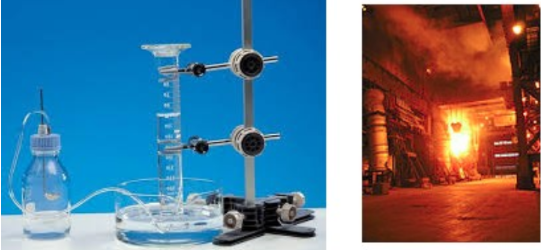
\includegraphics[width=0.25\textwidth]{./img/img00.png}
\end{wrapfigure} 
Pour pouvoir établir un diagnostic, le médecin peut
prescrire des analyses qui sont effectuées dans des
laboratoires spécialisés.
\textbf{Quelles sont les grandeurs indiquées sur le résultat d’une
analyse médicale ?}

%__________sub_Section 1 _______________
\section{La détermination de la quantité de matière d'un liquide ou solide :}
    \subsection{Définition de la quantité de matière :}
La quantité de matière est le nombre d’entités élémentaires dans un échantillon donnée. Par
exemple, le nombre de molécules, d’ions, d’atomes... .C'est une grandeur
notée : n , son unité est la mole , son symbole :(mol).
On appelle une mole de particules (atome, molécule ,ion ....etc ) l' ensemble de particules identiques.
$\mathscr{N_A}$ = 6,02.1023 est appelé : le nombre d'Avogadro.

Le nombre N d’atome, de molécules ou d’ions contenus dans l’échantillon est proportionnel à la
quantité de matière n correspondante. D’où la relation :$$n =\frac{N}{\mathscr{N_A}} $$
    \subsection{Relation entre la masse et la quantité de matière : }
    La quantité de matière contenue dans un échantion de masse m est donnée par la relation suivante: $$n = \frac{m}{M}$$
    n : la quantité de matière en (mol), \hspace{1cm} m : la masse en (g), \hspace{1cm} M : la masse molaire en (g/mol).

    Cette relation s'applique pour les solides les liquides (et même pour les gaz) mais il est plus commode de caractériser un gaz par son volume que par sa masse.\\
\underline{Exemple: }Déterminer la quantité de matière contenue dans 11,2g d'acide sulfurique $H_2SO_4$ .
\\On donne : M(H)=1g/mol , M(O)=16g/mol , M(S)=32g/mol.

\subsection{Relation entre le volume et la quantité de matière :}
La masse volumique : $\rho = \frac{m}{V}$ donc $m = \rho.V$ La relation devient : $$ n = \frac{\rho.V}{M}$$ avec M : la masse molaire (g/mol) et $\rho en (g/cm^3)$ et V en ($cm^3$)
\\Remarque : la densité d'un coprs solide ou liquide est liée $\grave{a}$ la masse volumique par la relation suivante : $$d = \frac{\rho}{\rho_{eau}}$$
donc la relation précédente : $$n = \frac{d.\rho_{eau}.V}{M}$$

%______________sub___Section 2_______________________________
\section{Détermination de la quantité de matière d'un gaz : }
\subsection{Le volume molaire : }
Le volume molaire VM , est le volume occupé par une mole de gaz dans les conditions normales de température et
de pression.
L'unité du volume molaire est (L/mol).
\\Dans les conditions normales de température et de pression : ($\theta = 0^{\circ}$ et P = 1 atm ) : $V_m = 22.4 L/mol$
\\Dans les conditions standards de température et de pression : ($\theta = 20^{\circ}$ et P = 1 atm ) : $V_m = 24 L/mol$

\subsection{Relation entre la quantité de matière d'un gaz et le volume molaire: }
La quantité de matière d'un gaz est donnée par la relation suivante:
$$n = \frac{V}{V_m}$$
avec n : quantité de matière en (mol) et V : le volume du gaz en (L) et $V_m$ : le volume molaire en (L/mol)


%______________sub___Section 2_______________________________

\section{Loi de Boyle Mariote : }
\begin{wrapfigure}{r}{0.25\textwidth}
    \centering
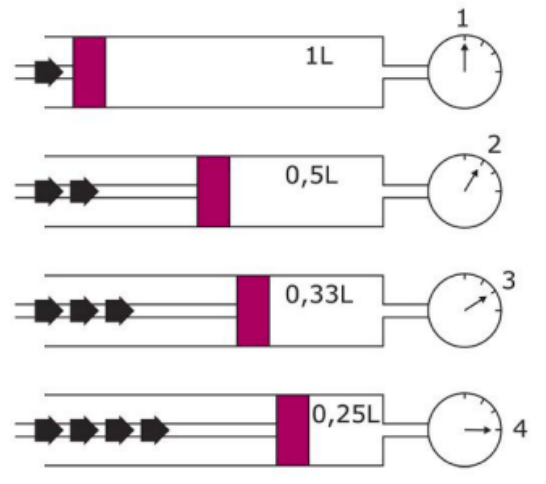
\includegraphics[width=0.25\textwidth]{./img/img01.png}
\end{wrapfigure} 

\subsection{Expérience : }
On considère une seringue remplie d’air et reliée à un manomètre
qui indique la pression P bar=1atm. On diminue le volume occupé par
l’air. On constate alors que la pression affichée par le manomètre
augmente.
Calculer le produit P.V

\subsubsection{Conclusion : }
Lorsque l’on diminue le volume d’air, la pression de ce gaz augmente.
Cependant le produit de la pression par le volume reste constant a
température constante.
On écrira alors la relation P.V = constante (à T constante).

Énonce de la loi :
À température constante, pour une quantité de matière donnée de gaz, le produit de la
pression P par le volume V de ce gaz ne varie pas :P×V = constante.

\subsection{La température absolue : }

On enferme une quantité d’air dans un ballon (n et V constants) On chauffe, puis on refroidit le
ballon et on note les valeurs de la température et la pression indiquées par les instruments de
mesure (manomètre digital et thermomètre a mercure) et on obtient le tableau suivant :
\begin{table}[h]
    \centering
\begin{tabular}{|c|c|c|c|c|c|}
    \hline
    $t(^{\circ})$ & -78 & 0   & 25   & 45   & 10\\\hline
    P(hPa)        & 676 & 940 & 1029 & 1100 & 1281\\\hline
\end{tabular}
\\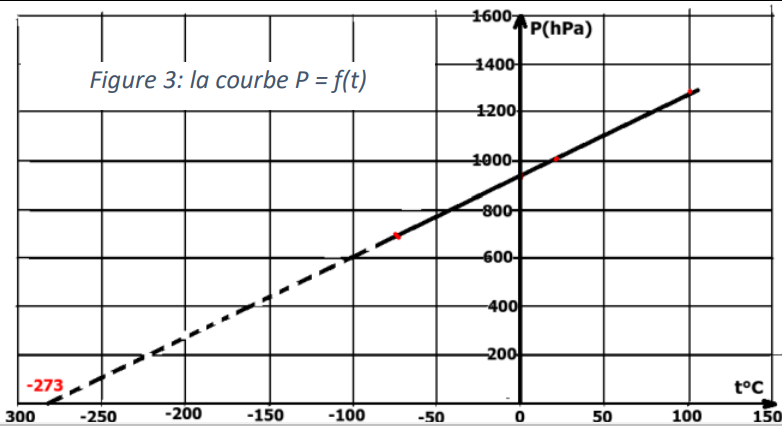
\includegraphics[width=0.5\textwidth]{./img/img02.png}
\end{table}\\
\\\underline{Exploitation : }
La courbe représentant la pression du gaz (air) en fonction de la température en Celsius, est
une droite passant par le point d’abscisse $-273^{\circ}C$ A cette température la pression du gaz s’annule mais en réalité la pression d’un gaz ne s’annule jamais.

Donc la température d’un gaz ne peut pas se descendre de $-273^{\circ}C$ et c’est pour cela ce point
s’appelle le zéro absolu.


Si on prend, pour une nouvelle courbe, l’origine $-273^{\circ}C$ on aura une nouvelle échelle appelée :
échelle absolue ou échelle Kelvin en remplaçant t$^{\circ}C$ par T exprimé en Kelvin (K) et la relation
entre ces deux échelles : $$T(K) = 273 +t(^{\circ}C)$$


\subsection{Relation des gaz parfaits : }
Un gaz est dit parfait si les interactions entre les molécules qui le constituent sont très faibles.
(donc les molécules d'un gaz parfait sont très éloignées entre elles par conséquence ,un gaz réel peut jouer le rôle
d'un gaz parfait à faible pression et haute température). $$P.V = n.R.T$$

P: la pression du gaz en pascal (Pa).
V: le volume du gaz en $m^3$.
n : la quantité de matière du gaz en (mol).
T : la température absolue du gaz en (K).
R : la constante des gaz parfait , sa valeur dans le système international est : R=8,314 J/mol.K.

\subsection{Densité d'un gaz par rapport à l'air :  }
La densité d'un gaz par rapport à l'air est égale au quotient de la masse d'un volume V du gaz par la masse du même
volume d'air.
$$d = \frac{m}{m_{air}}$$
On a $$\rho = \frac{m}{V} \rightarrow  m = \rho.V$$
alors $$d = \frac{m}{m_{air}} = \frac{\rho.V}{\rho_{air}.V} = \frac{\rho}{\rho_{air}}$$
D'autre part ,dans les mêmes conditions de températures et de pression (conditions normales par ex.) on a:
$$\frac{P}{RT} = \frac{n_{gaz}}{V} \; (1)$$
$$\frac{P}{RT} = \frac{n_{air}}{V} \; (2)$$
de (1) et (2) On a :  $$  \frac{n_{air}}{V}= \frac{n_{gaz}}{V}$$
donc : $  \frac{m_{air}}{M_{air}.V}= \frac{m_{gaz}}{M_{gaz}.V}$
et $\frac{\rho_{air}}{M_{air}}= \frac{\rho_{gaz}}{M_{gaz}}$
$$ d = \frac{\rho_{gaz}}{\rho_{air}} = \frac{M_{gaz}}{M_{air}}$$

Or la masse volumique de l'air dans les conditions normales de température et de pression est : $\rho_{air} = 1.293g/L$ et le volume molaire normale est : $V_M=22.4L/mol$, donc la masse molaire de l'air est : $M_{air} =\rho_{air}.V_{air}  = 1.293 . 22.4  = 29 L/mol$
donc la densité d'un gaz par rapport $\grave{a}$ l'air est : $$d = \frac{M_{gaz}}{29}$$

La densité d , est une gradeur sans unité 
\\M : mase molaire du gaz.
si $d>1$ le gaz est plus dense que l'air.
si $d<1$ le gaz est moins dense que l'air.
\\Exemples :
\\1) Calculer la densité du chlorure d’hydrogène HCl. Est il plus ou moins dense que l’air ?
\\2) Calculer la densité du dihydrogène H2. Est il plus ou moins dense que l’air ?
(on donne M(H)=1g/mol , M(Cl)=35,5g/mol .

\end{document}
